This project works on a layered data stack that handles big data, i.e., large volumes of structured and unstructured data types at a high velocity. The data stack handles how data is stored, managed, and retrieved to enable applications built on top of it. 
No single data stack applies to all cases, i.e., different approaches use different architectures \cite{framptonCompleteGuideOpen2018,sakrBigDataProcessing2017}. Therefore, this project defines a data stack and then focuses on the mainly two layers, i.e. the query engine and data management layer. The data stack of the project is illustrated in Figure \ref{fig:data_stack}.

\begin{figure}[!ht]
    \begin{center}
      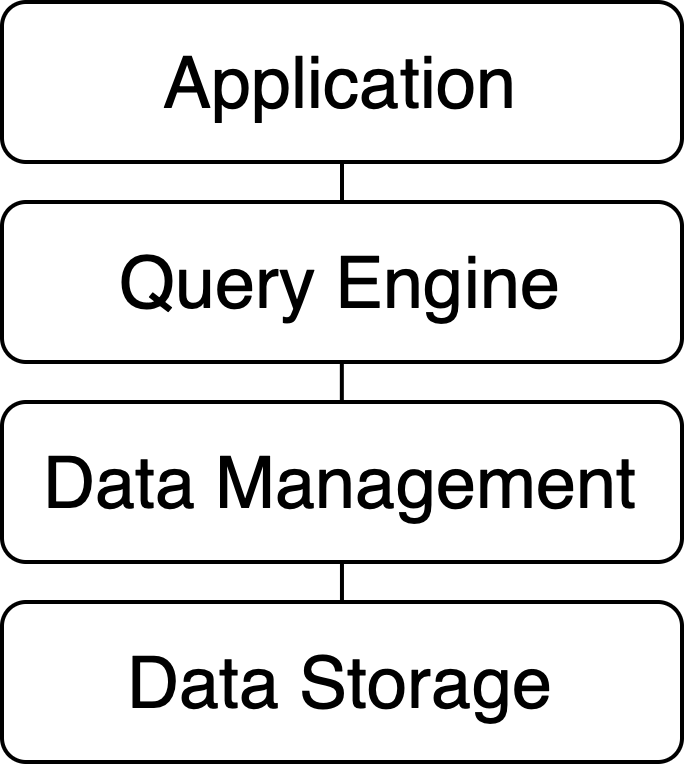
\includegraphics[width=0.4\textwidth]{figures/2-background/data_stack.png}
    \end{center}
    \caption[Data stack abstraction]{Data stack abstraction for this project.}
    \label{fig:data_stack}
\end{figure}
The data stack and this chapter are divided into four sections:
\begin{enumerate}
    \item \textbf{Data Storage}: handles how the data is stored. The data storage layer might be centralized or distributed, on-premise or in the cloud, and store data in files, objects, or blocks.
    \item \textbf{Data Management} : handles how the data is managed. The data management layer might offer \gls{ACID} properties, data versioning, support open data formats, and support structured and unstructured data.
    \item \textbf{Query Engine}: handles how data is queried, i.e., accessed, retrieved and written. The query engine might offer caching, highly scalable architectures, and \gls{API} support for multiple programming languages.
    \item \textbf{Application}: a system that will take advantage of the data stack. In the case of this project, only the software the Hopsworks feature store software will be described. 
\end{enumerate}
After explaining the data stack, a section on the legacy and new system architectures complements the Background, showing how the technologies explained function within the pipelines measured during the experiments.
%After explaining the data stack, a section on programming languages complements the Background by explaining the roles different programming languages play in the data stack (namely, Python, Java, and Rust).
